\documentclass[border=10pt]{standalone}
\usepackage[svgnames]{xcolor}
\usepackage{amsmath}
\usepackage{pgfplots}
\pgfplotsset{compat=newest}
\usepackage[sfdefault]{FiraSans}
\usepackage{FiraMono}
\renewcommand*\familydefault{\sfdefault}
\begin{document}
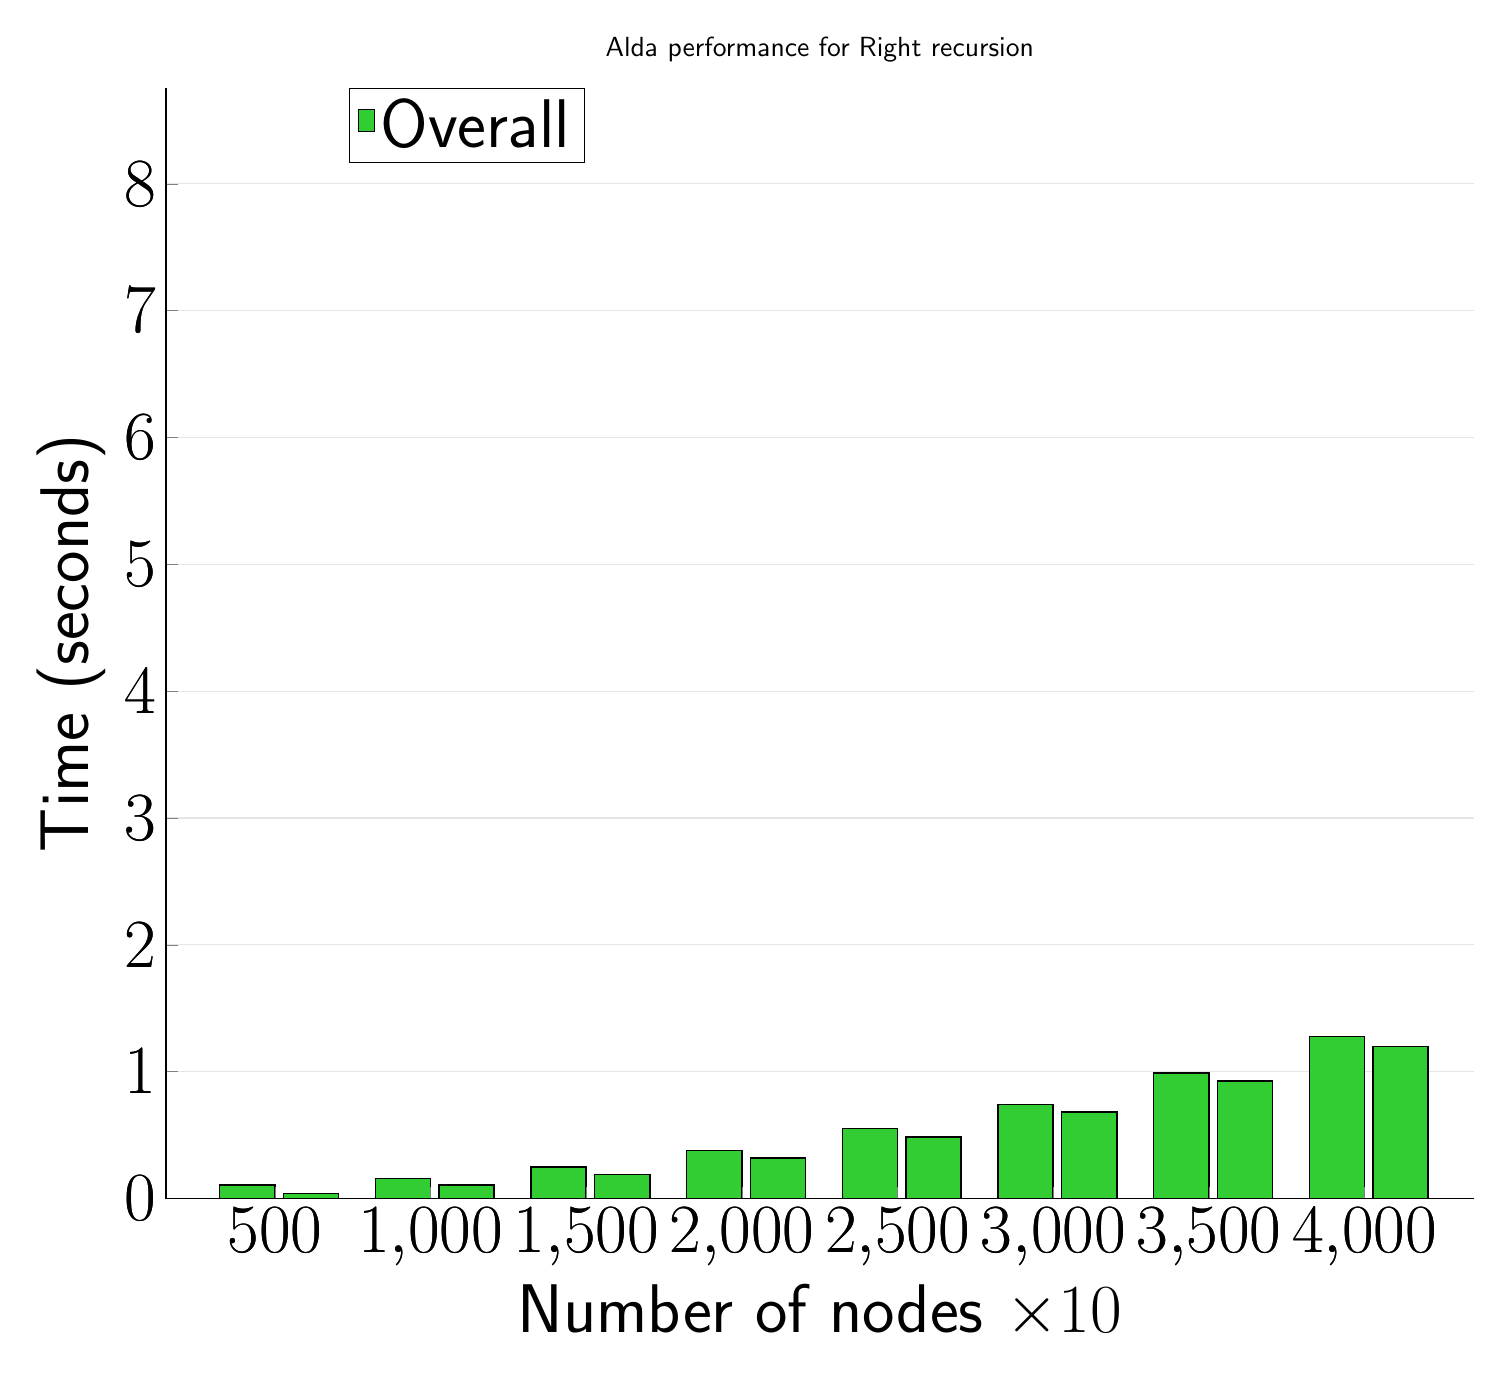
\begin{tikzpicture}
	\begin{axis}[
			ybar stacked,
			title={Alda performance for Right recursion},
			bar shift=-10pt,
			width=1.5\textwidth,
			bar width=0.7cm,
			ymajorgrids, tick align=inside,
			major grid style={draw=gray!20},
			xtick=data,
			ymin=0, ymax=8.757000017166138,
			axis x line*=bottom,
			axis y line*=left,
			enlarge x limits=0.1,
			legend style={
					at={(0.23, 1)},
					anchor=north,
					legend columns=1,
					font=\Huge,
				},
			ylabel={Time (seconds)},
			xlabel={Number of nodes $\times 10$},
			label style={font=\Huge},
			tick label style={font=\Huge},
		]
		\addlegendimage{fill=LimeGreen, draw=black, line width=0.2pt}
		\addlegendentry{Overall}
		\addplot +[fill=LimeGreen, draw=black, line width=0.5pt] coordinates {
				(500, 0.10700004100799561)
				(1000, 0.1570000171661377)
				(1500, 0.24800000190734864)
				(2000, 0.38100008964538573)
				(2500, 0.5509999752044678)
				(3000, 0.7440000057220459)
				(3500, 0.9900000095367432)
				(4000, 1.2769999980926514)
			};
	\end{axis}
	\begin{axis}[
			ybar stacked,
			bar shift=13pt,
			width=1.5\textwidth,
			bar width=0.7cm,
			ymajorgrids, tick align=inside,
			major grid style={draw=none},
			xtick=data,
			ymin=0, ymax=8.757000017166138,
			axis x line*=none,
			axis y line*=none,
			enlarge x limits=0.1,
			label style={font=\Huge},
			tick label style={font=\Huge},
		]
		\addplot +[fill=LimeGreen, draw=black, line width=0.5pt] coordinates {
				(500, 0.042)
				(1000, 0.10700000000000001)
				(1500, 0.19199999999999998)
				(2000, 0.31999999999999995)
				(2500, 0.4840000000000001)
				(3000, 0.6809999999999999)
				(3500, 0.9259999999999999)
				(4000, 1.1999999999999997)
			};
	\end{axis}
\end{tikzpicture}

\end{document}
